\newpage

\chapter{Desarrollo software }
\chaptermark{desarrollo}
\label{chap:desarrollo-software}

\section{Metodología de desarrollo}

Este proyecto ha sido elaborado empleando una metodología de desarrollo basada en el modelo de desarrollo incremental para la parte software referente a todos los subsistemas que
implican labores de programación, que son las referentes la programación de la placa Raspberry Pi y la programación de la placa Arduino.\\

El modelo de desarrollo incremental proporciona una serie de características que lo hacen idóneo para este proyecto. Dicho modelo se basa en la filosofía de construir 
e ir incrementando las funcionalidades del sistema mediante el desarrollo de los diferentes módulos. Esto permite ir aumentando gradualmente las capacidades del software. \\

Dicha metodología de desarrollo resulta especialmente útil en las siguientes situaciones:\\

\begin{itemize}
 \item Facilita el desarrollo permitiendo a cada miembro del equipo desarrollar un módulo particular. En el caso del presente proyecto me ha permitido desarrollar un módulo tras otro de una manera secuencial.
 \item Es similar al ciclo de vida en cascada aplicándose un ciclo en cada nueva funcionalidad del programa.
 \item A final de cada ciclo se entrega el software al cliente. En el caso que compete a este proyecto se mantenía una reunión con el director del proyecto para su aprobación.
\end{itemize}

Centrándonos nuevamente en el desarrollo del proyecto, los motivos que llevaron a cabo la elección de un modelo de desarrollo incremental viene dada por la necesidad de simplificar e ir
desarrollando de una forma gradual y modularizada debido a la extensión del proyecto. Más si cabe que el equipo de desarrollo solo consta de una persona.\\

Por tanto el proyecto queda distribuido en los siguientes subsistemas:\\

\begin{figure}[H]
  \begin{center}
    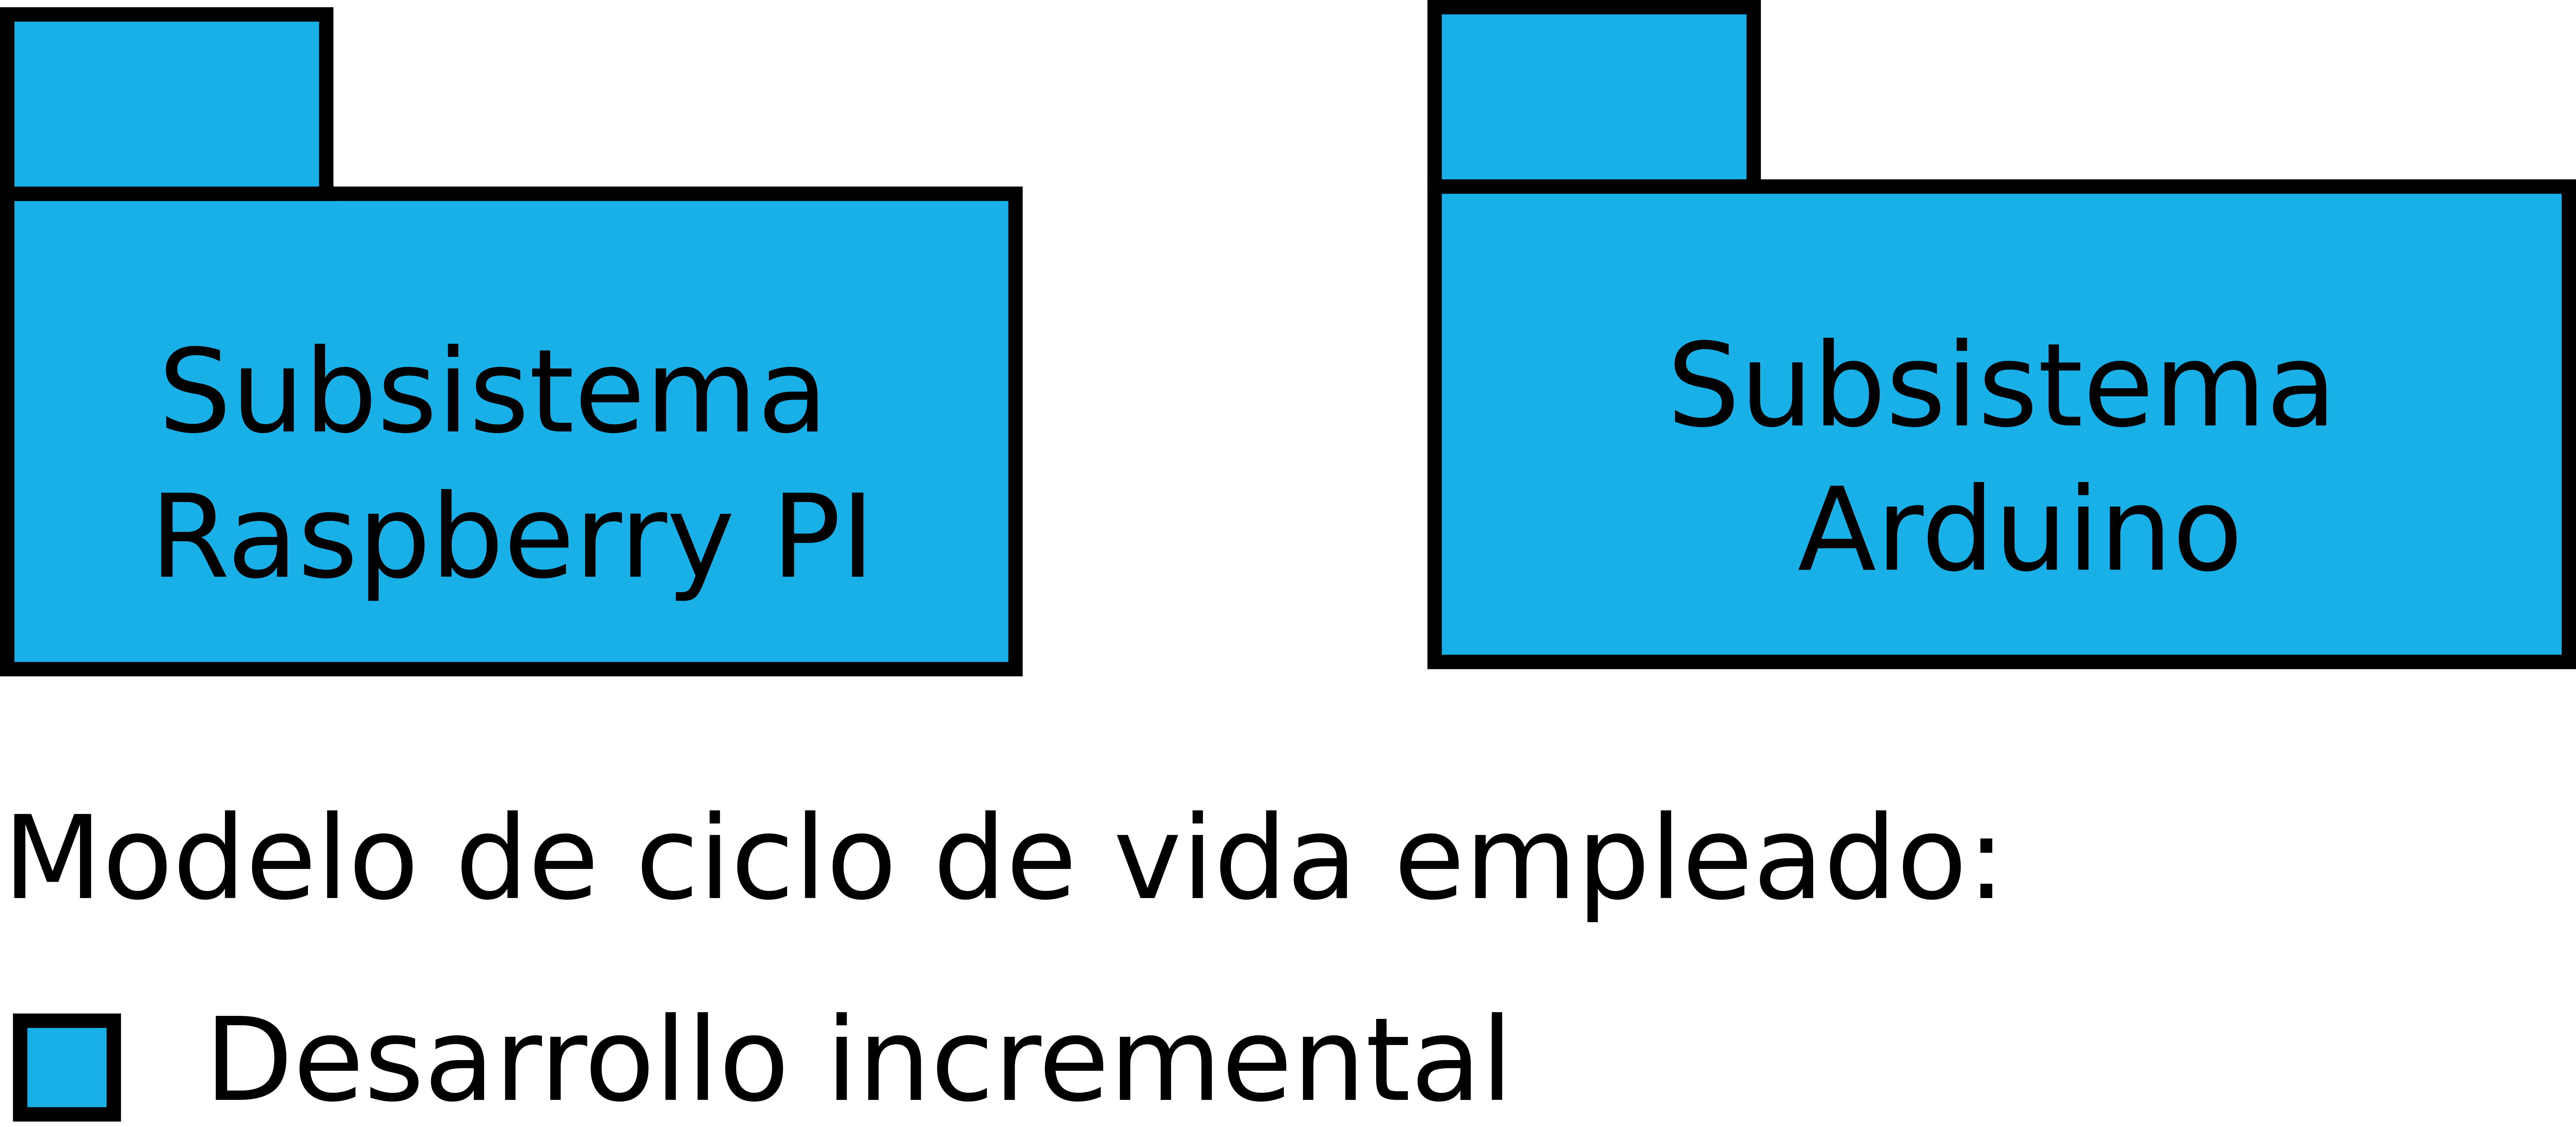
\includegraphics[scale=0.03]{diagramas/subsistemas.png}
  \end{center}
  \caption{Subsistemas existentes en el proyecto junto con el modelo de ciclo de vida
utilizado para su desarrollo.}
  \label{diagrama:subsistemas}
\end{figure}

Donde el subsistema Arduino abarca todas las tarear referentes a la programación del microcontrolador e interconexionado con todos los sensores utilizados y el subsistema Raspberry Pi
consta de todos aquellos porcesos de captación de datos, procesmiento y envío al servidor de control.\\

\subsubsection{Diagrama de casos de uso}

Una vez analizados los componentes hardware principales a utilizar, pasamos al análisis de los diferentes requerimientos funcionales para el vehículo a desarrollar.

\begin{figure}[H]
  \begin{center}
    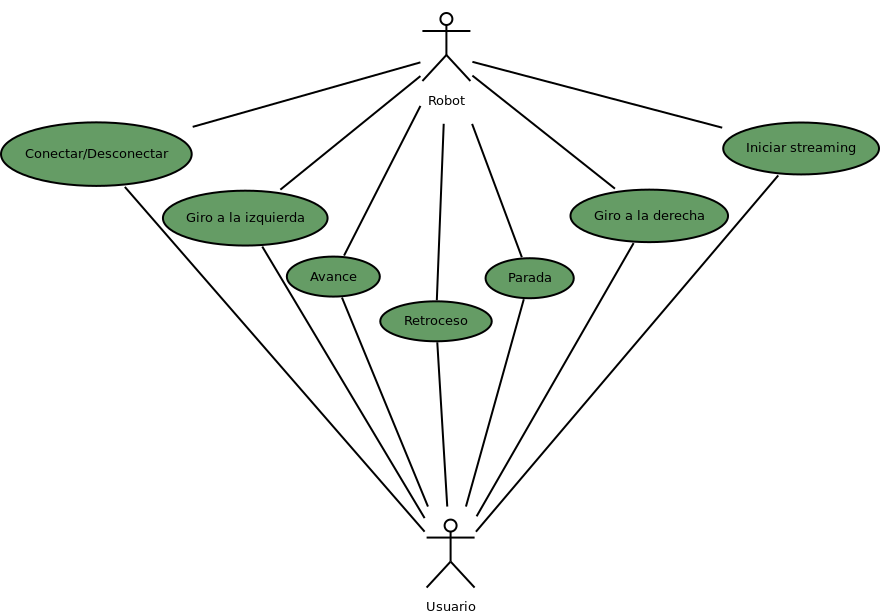
\includegraphics[scale=.4]{diagramas/casos-uso-robot.png}
  \end{center}
  \caption{Diagrama de casos de uso para la interacción con el robot.}
  \label{diagram:caso-uso}
\end{figure}

\subsubsection{Estados del robot}

Otro de los requerimientos es que el robot deberá de responder a una serie de estados de tal modo que en la aplicación se conozca las diferentes situaciones en la que se pueda encontrar un robot.
En el autómata diseñado encontramos un modo desactivado, modo de espera y modo de conexión. El autómata representativo es el siguiente:\\

\begin{figure}[H]
  \begin{center}
    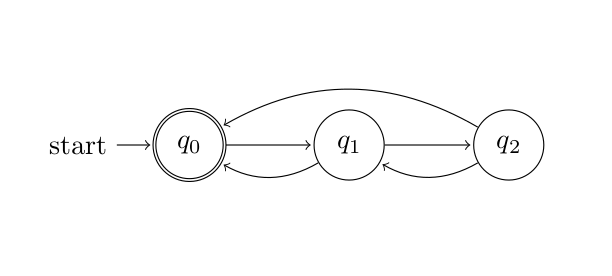
\includegraphics[scale=0.6]{imagenes/robot/automata-estados.png}
  \end{center}
  \caption{Autómata representativo de los diferentes estados del robot.}
  \label{figura:automata-estados}
\end{figure}

Donde:\\

\begin{itemize}
  \item Estado q0 inicial y final se corresponde con el estado apagado.
 \item Estado q1 se corresponde con el estado en escucha.
 \item Estado q2 se corresponde con el estado en funcionamiento.
\end{itemize}


\section{Software de control}
 
Para la programación de la placa Raspberry Pi se ha empleado el lenguaje de programación JavaScript en un entorno de ejecución Node.js para la que se han utilizado las siguientes 
bibliotecas o módulos:\\

\begin{itemize}
 \item \emph{pigpio}: Módulo para la comunicación y control de los pines GPIO de la Raspberry pi.
 \item \emph{child process}: El módulo child\_process proporciona la capacidad de generar procesos secundarios. Se ha empleado para la captura de vídeo mediante el lanzado de comandos ffmpeg.
 \item \emph{socket.io}: Biblioteca que establece enlaces bidireccionales en tiempo real y en comunicación basada por eventos.
 \item \emph{SerialPort} Módulo para la comunicación serie utilizado para establecer comunicación con la placa Arduino.
\end{itemize}


Por otra parte, para la programación de la placa Arduino se ha utilizado el legunaje de programación \emph{Arduino programming language} el cual está basado en C++ y aunque 
la referencia para el lenguaje de programación de Arduino se encuentra disponible en \url{http://arduino.cc/en/Reference/HomePage}, también es posible usar comandos estandar de C++ en la
programación de Arduino. Las bibliotecas Arduino utilizadas han sido las siguientes:\\

\begin{itemize}
 \item \emph{TonePlayer}: Biblioteca para la activación de los zumbadores.
 \item \emph{SimpleDHT}: Bibliotecaía para la lectura del sensor de temperatura y humedad del sensor DTH11 encontrándose la descripción en la sección \ref{sec:dth11}.
 \item \emph{NewPing}: Biblioteca para la lectura de los sensores de ultrasonido HC-SR04 cuya descripción se encuentra en la sección \ref{sec:ultrasonido}.
\end{itemize}


\section{Comunicación interna}

Para la comunicación entre elementos del dispositivo, como hemos estado comentando en diversas ocasiones, disponemos de dos módulos principales interconectados, uno de ellos es 
la placa Raspberry Pi, y el otro, la placa Arduino. En la presente sección se recogerán aquellos aspectos necesarios y de interés a nivel de programación para la comunicación entre elementos.\\

La Figura \ref{figura:diagrama-comunicacion-robot} corresponde con el diagrama de bloques de los diferentes canales de comunicaciones abiertos por SensorRS.\\

\begin{figure}[H]
  \begin{center}
    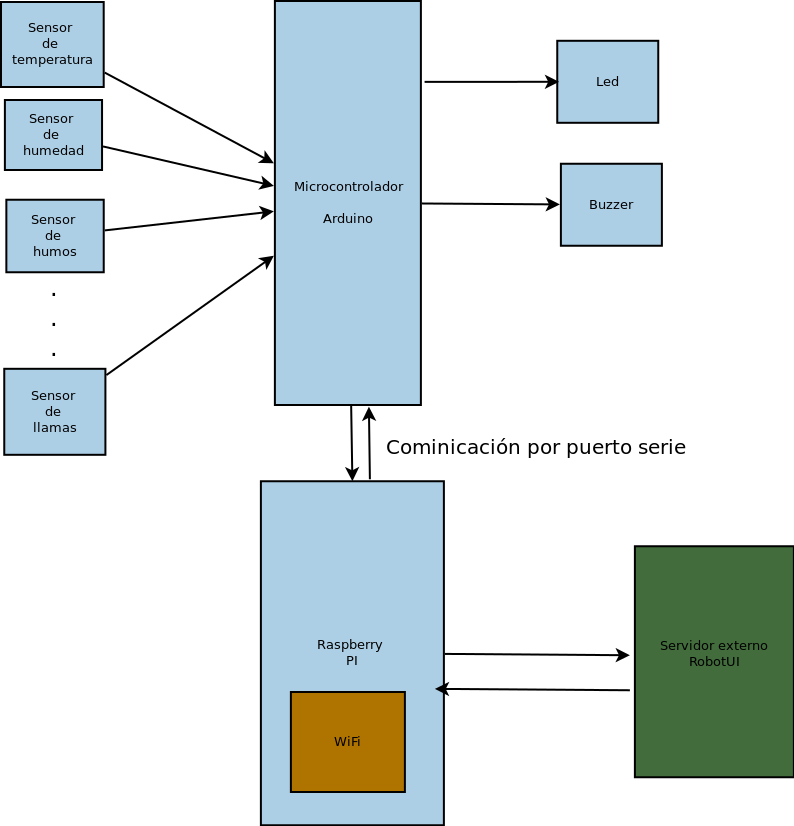
\includegraphics[scale=0.4]{diagramas/diagrama_bloques_robot.png}
  \end{center}
  \caption{Diferentes flujos de comunicación abiertos por SensorRS.}
  \label{figura:diagrama-comunicacion-robot}
\end{figure}

\subsection{Entrada/Salida Raspberry Pi}


En la presente sección se describen los diferentes canales de comunicación de entrada/salida utilizados en la Raspberry Pi para la comunicación con la Placa Arduino o el servidor de control.\\

\subsubsection{GPIO}

En esta ocasión no ha resultado necesario utilizar los pines GPIO que dispone la Raspberry Pi puesto que disponemos de los pines de entrada/salida que proporciona
el microcontrolador Arduino y han resultado suficientes.\\

Si, en cambio, para el vehículo que deseemos programar resultan necesarios más pines para la utilización de servos, sensores o cualquier otro elemento extra que utilize los pines
GPIO de la placa Raspberry Pi, tan solo debemos inicializarlos e indicar si van a ser pines de entrada o de salida. Si existen dudas al respecto se puede acceder a la documentación de
la biblioteca \emph{pigpio} en el siguiente enlace: \url{https://www.npmjs.com/package/pigpio}.\\

Un posible ejemplo sería la inicialización de unos pines para una controladora de motores L298N que en lugar de conectarla a la placa Arduino la hubésemos conectado directamente a 
la placa Raspberry Pi:\\

\begin{lstlisting}[language=JavaScript]
  // Carga del módulo.
  var Gpio = require('pigpio').Gpio;

  // Pines utilizados. Motores izquierdos: 2 y 3, motores derechos: 17 y 27
  var gpio2 = new Gpio(2, {mode: Gpio.OUTPUT}),
    gpio3 = new Gpio(3, {mode: Gpio.OUTPUT}),
    gpio17 = new Gpio(17, {mode: Gpio.OUTPUT}),
    gpio27 = new Gpio(27, {mode: Gpio.OUTPUT}),
    gpio4 = new Gpio(4, {mode: Gpio.INPUT, alert: true});
\end{lstlisting}


Para la escritura o lectura en los puertos inicializados utilizamos las siguiente sentencias:\\

\begin{lstlisting}[language=JavaScript]
  gpio2.digitalWrite(1);  //Escritura en pin 2
  
  gpio4.on('alert', (level, tick) => {
    console.log('Activo!');
  });  //Activacion del evento tras activación del pin 4
\end{lstlisting}


\subsubsection{comunicación Serie}
\label{subsec:raspberry_serie}

La comunicación serie mediante el uso del puerto USB se ha utilizado para la interconexión entre la placa Raspberry Pi y Arduino con la finalidad de transmitir información referente
a las mediciones realizadas por los sensores y control de los mismos.\\

Para establecer dicha comunicación hemos utilizado el módulo JavaScript \emph{SerialPort} resultando necesario conocer y especificar el puerto serie asignado a nuestra placa Arduino. 
Para ello abrimos una terminal en nuestra Raspberry Pi con la placa Arduino previamente conectada e introducimos el siguiente comando:\\

\begin{lstlisting}[language=bash]
ls /dev | grep ttyACM
\end{lstlisting}

Una vez conocido el puerto, en nuestro caso \emph{/dev/ttyACM0}, lo emplearemos para la inicialización de la conexión con el puerto serie.\\

\begin{lstlisting}[language=JavaScript]
    // Carga del módulo.
    const SerialPort = require('serialport');
    const Readline = SerialPort.parsers.Readline;
    const port = new SerialPort('/dev/ttyACM0', {
      baudRate: 9600
    });
    
    const parser = new Readline();
    port.pipe(parser);
\end{lstlisting}


A continuación, se muestra el código implementado para el envío de datos a la placa Arduino \empg{serial\_transmission} junto con la inicialización del puerto y carga de las librerías:\\

\begin{lstlisting}[language=JavaScript]

function serial_transmission( data, delay ){
  setTimeout(function() {
    // Envío del string caracter por caracter
    for(var i=0; i<data.length; i++){
      port.write(new Buffer(data[i], 'ascii'));
    }
    // Envío del caracter final \n
    port.write(new Buffer('\n', 'ascii'));

  }, delay  );

}
\end{lstlisting}

Como se observa en la función superior la transmisión de información se realiza transmitiendo la cadena deseada caracter por caracter introduciendo finalmente un caracter identificador de final de línea que,
para nuestro caso, hemos empleado el '\n' indicativo de salto de línea.\\

El envío de cada caracter irá acompañado de un retraso, \emph{delay}, el cual es introducido por parámetro a la función.\\

Para la captación por parte de la Raspberry Pi de los parámetros emitidos por la Placa Arduino se dispone de la siguiente función:\\

\begin{lstlisting}[language=JavaScript]
  const parser = port.pipe(new Readline({ delimiter: '\r\n' }));
  parser.on('data', function(data){
    console.log(data);
    var msg_data = data.split("%");
    socket.emit(String(msg_data[0]), {msg: String(msg_data[1]) } );
  });

\end{lstlisting}

Dicha función se encarga de una vez capturado el mensaje, romperlo en dos secciones delimitadas por el caracter '\%' siendo la parte izquierda (almacenada en msg_data[0]) la referente al tipo de dato recibido
y la derecha (almacenada en msg_data[1]) el propio valor del mensaje. Por ejemplo, para el sensor de temperatura tenemos el identificador \emph{tmp} siendo un posible mensaje
resultante \emph{tmp\%22 *C}.\\

Finalmente se realiza el envío del dato a través del websocket al servidor de control, donde el nombre del evento se corresponde con el nombre del tipo de dato recibido con la sentencia \emph{Socket.emit}.\\

\subsection{Entrada/Salida Arduino}

\subsubsection{Lectura puerto serie}

A continuación se muestra una sección del código destinado a la recepción de un mensaje enviado desde la placa Raspberry Pi. El ejemplo mostrado recibe los comando necesarios para
la activación de los motores:\\

\begin{lstlisting}[language=C++]

#define E1 10  // Enable Pin motor 1
#define I1 8  // Control pin 1 motor 1
#define I2 9 // Control pin 2 motor 1

void setup() {
  Serial.begin(9600); //Seteo de la tasa de transferencia

  pinMode(E1, OUTPUT);
  pinMode(I1, OUTPUT);
  pinMode(I2, OUTPUT);

  pinMode(E2, OUTPUT);
  pinMode(D2, OUTPUT);
  pinMode(D1, OUTPUT);

  // Seteo de direccion de rotación inicial
  digitalWrite(I1, LOW);
  digitalWrite(I2, HIGH);
  digitalWrite(D1, LOW);
  digitalWrite(D2, HIGH);
}

void loop() {


  while (Serial.available() > 0) {
    char received = Serial.read();
    inData.concat(received);

    if (received == '\n') {
      inData.trim();

      //MOTOR
      if (inData.startsWith("MOTOR")){
          if (sscanf(inData.c_str(), "MOTOR-%d", &motor) == 1) {
            Serial.println(motor);
          }

          if( motor <= 51 && motor >= -51 ){
            Serial.println('STOP');
            digitalWrite(E1, LOW);
            digitalWrite(I1, LOW);
            digitalWrite(I2, LOW);
          }

          if( motor > 51){
            analogWrite(E1, motor);
            digitalWrite(I1, HIGH);
            digitalWrite(I2, LOW);
          }

          if( motor < -51 and ! stop){
            motor = motor * -1;
            analogWrite(E1, motor);
            digitalWrite(I1, LOW);
            digitalWrite(I2, HIGH);
          }
      }
      inData = "";
    }
  }
 
  delay(100);

}
\end{lstlisting}


Como podemos observar en el código superior, la función consta de un bucle principal que va leyendo los diferentes caracteres que recibe concatenándolos en una variable hasta recibir 
el caracter utilizado como indicativo de final de mensaje '\textbackslash n'. Por lo que el mensaje quedaría interceptado e interpretado como completo. El código 
análogo de la Raspberry Pi se localiza en la sección \ref{subsec:raspberry_serie}.\\

Centrándonos nuevamente en el ejemplo superior, se recibe la palabra clave \emph{MOTOR-} seguida del valor de la velocidad de giro, siendo éstas positivas, avance o negativas para el retroceso en un rango
que abarca entre los -255 a 255 y delimitado por '\textbackslash n'. Por lo que si el mensaje cumple el patrón deseado activará las salidas correspondientes a la acción a realizar.\\

Otro punto a destacar es que los valores de detección del motor se encuentran en el rango situado entre -51 y 51. Ésto es debido a que a velocidades muy pequeñas el motor no aquiere la
suficiente fuerza como para traccionar el vehículo evitando así consumos inecesarios y ruido ocasionado por los motores.\\

\subsubsection{Escritura en puerto serie}

A continuación se muestra un ejemplo de envío de los valores de temperatura y humedad del sensor Dth11 conectado al Arduino para su transferencia a la Placa Raspberry Pi:\\

\begin{lstlisting}[language=C++]
#include <SimpleDHT.h>

int pinDHT11 = 4;
String inData = "";

SimpleDHT11 dht11;

void setup() {
  Serial.begin(9600);
}

void loop() {
  byte temperature = 0;
  byte humidity = 0;
  int err = SimpleDHTErrSuccess;
  if ((err = dht11.read(pinDHT11, &temperature, &humidity, NULL)) != SimpleDHTErrSuccess) {
     Serial.print("Read DHT11 failed, err="); Serial.println(err);delay(1000);
  }

  dht11.read(pinDHT11, &temperature, &humidity, NULL);

  if ( (int)temperature != 0 and (int)humidity != 0 ){
    Serial.print("tmp%");
    Serial.print((int)temperature); Serial.print(" *C, ");
    Serial.print((int)humidity); Serial.println(" H");
  }

  
  delay(30);

  Serial.println(analogRead(photosensorPin));
}

\end{lstlisting}

Como podemos observar en el código superior, el mensaje transmitido presenta el siguiente formato: tmp\% xx*C xxH, donde \emph{tmp} representa el tipo de dato transmitido actuando el caracter '\%' como 
delimitador entre el tipo de dato y el dato en sí mismo.\\


\section{Comunicación externa}

En el punto anterior hemos visto las diferentes configuraciones de Entrada/Salida establecidas tanto para para el control de los diferentes motores y sensores en Arduino y Raspberry Pi. 
En el presente y sucesivos puntos describiremos los diferentes canales de comunicación abiertos y los flujos de información existentes entre la placa Raspberry Pi y el servidor de control donde 
se encuentra alojada la aplicación web para monitorización del vehículo SensorRS.\\

En la figura \ref{figura:comunicaciones-robot} se muestra un gráfico representativo de los diferentes flujos de datos existentes:

\begin{figure}[H]
  \begin{center}
    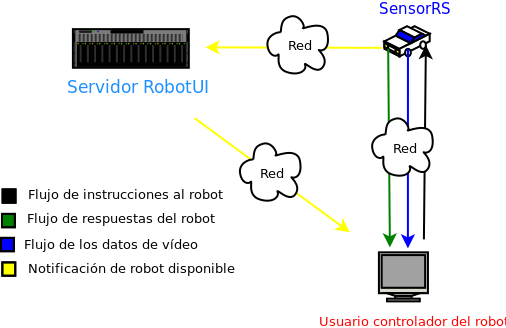
\includegraphics[scale=0.6]{diagramas/flujo-comunicaciones-robot.png}
  \end{center}
  \caption{Canales de comunicación abiertos externos a SensorRS.}
  \label{figura:comunicaciones-robot}
\end{figure}

Primeramente al accionar el robot, éste envía una notificación al servidor indicando que se encuentra en modo \emph{online} y permanece a la espera de que algún usuario de la aplicación decida
conectarse para su control. Canal de comunicación representado en amarillo en la figura \ref{figura:comunicaciones-robot}.\\

Un usuario ve disponible el robot y decide conectarse. Entonces se establece un enlace entre el robot, servidor, y el usuario, cliente. Flujo de comunicación representado en negro, figura \ref{figura:comunicaciones-robot}.\\

El usuario envía comandos al robot a través del canal abierto y las respuestas son enviadas a al cliente, transmisiones representados en verde para datos y en azul para el vídeo, figura \ref{figura:comunicaciones-robot}.\\

Las tres vías de comunicación entre el robot y el usuario discurren dentro de un mismo canal de comunicación (socket). En el siguiente punto se describirá más detalladamente el procedimiento.

\subsubsection{Sockets}

Ahora bien, una vez definidos los pines o comandos que derivaremos a la placa Arduino y que activarán nuestros motores o sensores y los canales de comunicación necesarios, necesitamos que éstos sean activados
cuando desde una red externa lo indiquemos. Para ello haremos uso de la biblioteca Socket.io. \\

Comenzamos el código incluyendo las librerías necesarias:\\

\begin{lstlisting}[language=JavaScript]
  var io_client = require('./node_modules/socket.io-client');
  var sails_client = require('./node_modules/sails.io.js');
\end{lstlisting}

Para la comunicaciones usuario y dispositivo robótico se ha empleado la biblioteca socket.io-client.\\

Para las comunicaciones directas con el servidor se ha empleado el SDK\footnote{Un kit de desarrollo de software o SDK (siglas en inglés de software development kit) es generalmente un conjunto de herramientas
de desarrollo de software que le permite al programador o desarrollador de software crear aplicaciones para un sistema concreto, por ejemplo ciertos paquetes de software, frameworks, etc.} proporcionado por el framework
para comunicarse con Sails a través de sockets desde una aplicación Node.js o desde el propio navegador.\\


El siguiente paso una vez cargadas las librerías es establecer las diferentes conexiones. El primer comportamiento deseado es, por parte del robot, lanzar un mensaje al servidor indicando su disponibilidad al servidor con la finalidad de
enviar las diferentes notificaciones a los usuarios que estén usando la aplicación. Para ello establecemos la conexión y enviamos un mensaje al servidor con el identificador del robot junto con su estado online igual a true. A continuación mostramos
el código:\\

\begin{lstlisting}[language=JavaScript]
  var io_server = sails_client(io_client);
  io_server.sails.url = 'http://46.101.102.33:80';
  io_server.socket.get('/robot/changetoonline/', {robot: '59188631c8e94ba54f7a4bdc', online: true});
\end{lstlisting}

Una vez realizado el paso anterior, tenemos al robot SensorRS que ha indicado a la aplicación web que se encuentra en estado online pero nada más. El siguiente paso sería establecer alguna 
comunicación que se mantuviera a la escucha a la espera de la llegada de nuevas conexiones. Para la creación del socket basta con la siguiente instrucción, la cual recibe un puerto que 
utilizará para mantenerse a la escucha:\\

\begin{lstlisting}[language=JavaScript]
  var io = require('./node_modules/socket.io').listen(8085, { log: false });
\end{lstlisting}


Con la finalidad de ir capturando los diferentes eventos, se han definido las siguientes funciones para la conexión y desconexión de los clientes:\\

\begin{lstlisting}[language=JavaScript]

io.sockets.on('connection', function (socket)
{

  //Almacenamiento del número total de clientes conectados.
  sockets[socket.id] = socket;
  console.log("Total clientes conectados : ", Object.keys(sockets).length);
  
  //Envío de un saludo.
  socket.emit('robotmsg', {msg: "!!!HOLA!!!"});


  //Salida de un cliente.
  socket.on('disconnect', function() {
    console.log('Bye!');
    stopStreaming(socket);
  });  
  
}
\end{lstlisting}

Cuando un evento \emph{action} es recibido se activada la función que procesa el comando recibido y activa las salidas correspondientes, la cual establece los pines necesarios a los valores
1 o 0 según el parámetro establecido.\\

\subsubsection{ Streaming de vídeo }

Para realizar la transferencia de vídeo desde el robot hacia el cliente se ha empleado la librería FFmpeg \footnote{ Los conocimientos necesarios para la comprensión de la herramienta FFmepg y sus modos de 
utilización se han adquirido accediendo a la documentación disponible en la referencia \cite{website:7} correspondiente con la documentación oficial.} haciendo uso de su herramienta de línea de comandos.\\

El procedimiento de captura de vídeo y su posterior transmisión es realizado mediante la siguiente instrucción de Ffmpeg:\\

\begin{lstlisting}[language=bash]
  ffmpeg -f video4linux2 -i /dev/video0 -s 300x150 -f mjpeg pipe:1 -b:v 28k -bufsize 28k
\end{lstlisting}

En los puntos sucesivos analizaremos qué es lo que realiza la instrucción anterior y por qué resulta clave en todo el proceso de difusión, comprendido desde la captura del 
vídeo hasta su posterior transmisión al usuario que está controlando el robot.\\

Nada prodríamos transmitir si no disponemos inicialmente de los datos que queremos difundir. De ahí que inicialmente debamos realizar la captura de las diferentes imágenes a partir de la cámara
USB conectada a la Raspberry Pi. Para ello se utiliza la API de captura de vídeo video4linux2 \footnote{ Video4Linux o V4L es una API de captura de video para Linux. Muchas webcams USB, sintonizadoras
de tv, y otros periféricos son soportados. Video4Linux está integrado con el núcleo Linux. V4L está en su segunda versión (V4L2). El V4L original fue incluido en el ciclo 2.1.X de desarrollo del
núcleo Linux. Video4Linux2 arregla algunos fallos y apareció en los núcleos 2.5.X. } (o simplemente v4l2) la cual dispone las bibliotecas de Ffmpeg. Tan solo debemos especificar el dispositivo de 
captura.\\

El nombre del dispositivo de captura es un nodo de dispositivo de archivo, por lo general los sistemas Linux tienden a crear automáticamente estos nodos cuando el dispositivo
está conectado al sistema, y ​​tiene un nombre del tipo /dev/videoN, donde N es un número asociado al dispositivo.\\ 


Para proceder a la captura de las imágenes nos bastaría con introducir el siguiente comando:\\

\begin{lstlisting}[language=bash]
  ffmpeg -f video4linux2 -i /dev/video0 -s 300x150 -f mjpeg video_out.mpeg
\end{lstlisting}

Ahora bien, el comando anterior toma las imágenes de la cámara y las almacena en el archivo especificado \emph{ video\_out.mpeg} especificando una resolución de salida de 300x150 píxeles
empleando la opción -s. Pero nosotros no deseamos exactamente ese comportamiento. Debemos canalizar esos datos capturados hacia el socket creado con la finalidad de ir transmitiendo los 
diferentes frames y no almacenándolos en disco tal y como realiza la instrucción anterior.\\


Para resolver este problema podemos emplear el sistema de tuberías que implementan los sistemas UNIX \footnote{ Una tubería (pipe, cauce o '|') consiste en una cadena de 
procesos conectados de forma tal que la salida de cada elemento de la cadena es la entrada del próximo. Permiten la comunicación y sincronización entre procesos. Es común el uso de
buffer de datos entre elementos consecutivos. }.\\

En cualquier sistema Unix se puede hacer que la salida de una determinada orden sea la entrada estándar de otra, lo que le confiere a las órdenes Unix una enorme potencia.
Para realizar dicha "canalización`` debemos utilizar las siguientes opciones:\\

\begin{lstlisting}[language=bash]
  pipe:1 -b:v 28k -bufsize 28k
\end{lstlisting}


Con la opción \emph{pipe:1} accedemos al protocolo pipe de UNIX, el cual lee y escribe de las \emph{tuberias} UNIX siendo el número 1 la tubería correspondiente a la salida estándar 
stdout ( 0 para stdin y 2 para stderr), la cual podría ser omitida puesto que es la salida por defecto.\\

La opción \emph{-b:v 28k} establece la tasa de transferencia, en nuestro caso una tasa de 28 kbit/s.\\

La opción \emph{-bufsize 28k} establece un tamaño de buffer \footnote{Un buffer de datos es un espacio de la memoria en un disco o en un instrumento digital reservado para el almacenamiento
temporal de información digital, mientras que está esperando ser procesada.} de 28 kbits.\\

A continuación mostramos el código de transmisión de vídeo al completo junto con la captura de los diferentes eventos activados cuando se produce la salida de datos por cada una de las salidas estándar:\\

\begin{lstlisting}[language=JavaScript]

  function startStreaming(socket) {
    //ffmpeg -f video4linux2 -i /dev/video0 -s 300x150 -f mjpeg pipe:1 -b:v 28k -bufsize 28k

    if (running_camera == false){
      console.log('Starting streaming....');
      var args = ["-f", "video4linux2", "-i", "/dev/video0", "-s", "300x150","-f","mjpeg", "pipe:1", "-b:v 28k", "-bufsize 28k"]
      ffmpeg_command = require('child_process').spawn("ffmpeg", args);
      running_camera = true
    }

    ffmpeg_command.on('error', function(err, stdout, stderr) {
      console.log("ffmpeg stdout:\n" + stdout);
      console.log("ffmpeg stderr:\n" + stderr);
      running_camera = false
    });


    ffmpeg_command.on('close', function (code) {
      console.log('ffmpeg exited' + code );
      running_camera = false
    });


    ffmpeg_command.stderr.on('data', function (data) {
      //console.log('stderr: ' + data);
    });

    ffmpeg_command.on('end', function() {
      console.log('Finished');
      running_camera = false
    });

    ffmpeg_command.stdout.on('data', function (data) {
      //console.log('stdout: ' + data);
      var frame = new Buffer(data).toString('base64');
      socket.emit('canvas',frame);
    });
  }

\end{lstlisting}


\subsubsection{Código de ejemplo completo}

Finalmente se muestra el código completo para el robot SensorRS desarrollado. Dicho código puede emplearse como guía de referencia o plantilla para futuros proyectos con la idea de integrarlos en la aplicación RobotUI.\\


\begin{lstlisting}[language=JavaScript]
var io_client = require('./node_modules/socket.io-client');
var sails_client = require('./node_modules/sails.io.js');
var io_server = sails_client(io_client);
io_server.sails.url = 'http://46.101.102.33:80';
io_server.socket.get('/robot/changetoonline/', {robot: '59188631c8e94ba54f7a4bdc', online: true});

// Inicia servidor socket.io en el puerto 8085.
var io =io_client.listen(8085, { log: false });

// Carga de módulos necesarios.
var ffmpeg_command, running_camera = false, child_process = require('child_process');

var Gpio = require('pigpio').Gpio;
// Pines utilizados. Motores izquierdos: 2 y 3, motores derechos: 17 y 27
var gpio2 = new Gpio(2, {mode: Gpio.OUTPUT}),
  gpio3 = new Gpio(3, {mode: Gpio.OUTPUT}),
  gpio17 = new Gpio(17, {mode: Gpio.OUTPUT}),
  gpio27 = new Gpio(27, {mode: Gpio.OUTPUT});


console.log('Esperando conexión...');

var sockets = {};

io.sockets.on('connection', function (socket)
{

  sockets[socket.id] = socket;
  console.log("Clientes totales conectados: ", Object.keys(sockets).length);

  socket.on('disconnect', function() {
    console.log('¡Adios!');
    //stopStreaming(socket);
  });


  socket.on('start-stream', function() {
    startStreaming(socket);
  });

  socket.emit('robotmsg', {msg: "¡¡¡Bienvenido!!!"});
  console.log('emitiendo: ' + "¡¡¡Bienvenido!!!");

  socket.on('action', function (data){
    console.log('Comando recibido: ' + data);
  });
  
});

function stopStreaming(socket) {
  delete sockets[socket.id];
  // no more sockets, kill the stream
  if (Object.keys(sockets).length == 0) {
    if (ffmpeg_command){
      ffmpeg_command.kill();
      running_camera = false;
      console.log('Stop streaming');
    }
  }
}

function startStreaming(socket) {
  //ffmpeg -f video4linux2 -i /dev/video0 -s 300x150 -f mjpeg pipe:1 -b:v 28k -bufsize 28k

  if (running_camera == false){
    console.log('Starting streaming....');
    var args = ["-f", "video4linux2", "-i", "/dev/video0", "-s", "300x150","-f","mjpeg", "pipe:1", "-b:v 28k", "-bufsize 28k"]
    ffmpeg_command = child_process.spawn("ffmpeg", args);
    running_camera = true
  }

  ffmpeg_command.on('error', function(err, stdout, stderr) {
    console.log("ffmpeg stdout:\n" + stdout);
    console.log("ffmpeg stderr:\n" + stderr);
    running_camera = false
  });


  ffmpeg_command.on('close', function (code) {
    console.log('ffmpeg exited' + code );
    running_camera = false
  });


  ffmpeg_command.stderr.on('data', function (data) {
    //console.log('stderr: ' + data);
  });

  ffmpeg_command.on('end', function() {
    console.log('Fin');
    running_camera = false
  });

  ffmpeg_command.stdout.on('data', function (data) {
    //console.log('stdout: ' + data);
    var frame = new Buffer(data).toString('base64');
    socket.emit('canvas',frame);
  });

}

\end{lstlisting}

Para la ejecución del código introducimos el siguiente comando:\\

\begin{lstlisting}[language=bash]
  sudo node raspberry.js
\end{lstlisting}

Siendo \emph{raspberry.js} el nombre del archivo que contiene nuestro código.\\

